\documentclass[a4paper, 11pt]{article}
\usepackage{amsmath, amssymb, amsthm}
\usepackage{xeCJK}
\usepackage{fontspec}
\usepackage{xunicode}
\usepackage{xltxtra}
\usepackage{graphicx}

\setCJKfamilyfont{tt}{SimSun}
\setmainfont{SimSun} 		%默认字体,默认英文字体。
\setCJKmainfont{SimSun} 		%中文默认字体
\setCJKmonofont{SimSun}
\CJKsetecglue{} 			%中英间隔

%\XeTeXlinebreaklocale "zh"  % 表示用中文的断行
%\XeTeXlinebreakskip = 0pt plus 1pt % 多一点调整的空间设置字体。

\newcommand{\cn}{\fontspec{Courier New}}
%字体大小
\newcommand{\ltwo}{\fontsize{18pt}{27pt}\selectfont} 		%小二
\newcommand{\three}{\fontsize{16pt}{24pt}\selectfont}		%三号
\newcommand{\lthree}{\fontsize{15pt}{22.5pt}\selectfont}	%小三
\newcommand{\four}{\fontsize{14pt}{21pt}\selectfont}		%四号
\newcommand{\lfour}{\fontsize{13pt}{18pt}\selectfont}		%小四
\newcommand{\five}{\fontsize{10.5pt}{15.75pt}\selectfont}	%五号
\newcommand{\lfive}{\fontsize{9pt}{13.5pt}\selectfont}		%小五

\usepackage{listings}
\lstset{language=Java}%这条命令可以让LaTeX排版时将C++键字突出显示
\lstset{breaklines}%这条命令可以让LaTeX自动将长的代码行换行排版
%\lstset{extendedchars=false}%这一条命令可以解决代码跨页时,章节标题,页眉等汉字不显示的问题
\lstset{xleftmargin=28pt}
\lstset{tabsize=4}
\lstset{escapechar=`} %中文注释问题
\lstset{columns=flexible}
\lstset{basicstyle=\cn\lfive}

%图,表标题的间距。
\usepackage{caption}
\setlength{\abovecaptionskip}{10pt}
\setlength{\belowcaptionskip}{0pt}
\usepackage{tabularx}

\renewcommand {\tablename}{\five 表}
\renewcommand {\thetable}{\arabic{table}}
\usepackage{booktabs}
\renewcommand {\heavyrulewidth}{1.5pt}	%表格外线宽
\renewcommand {\lightrulewidth}{1pt}	%表格内线宽

\captionsetup{labelsep=space}

%%%%%%%%%%%%%%%%%%%%%%%%
%%%%%%%%%%%正文%%%%%%%%%%
%%%%%%%%%%%%%%%%%%%%%%%%
\begin{document}

\title{{\Huge 算法分析与设计第四次作业\\}}
\author{黄丛宇 2010212439}
\date{\today}

\maketitle

\section{实验环境}
\begin{itemize}
	\item CPU: Intel(R) Core(TM)2 Duo CPU T5870 2.00GHz
	\item MEM: 1GB
	\item OS : Debian 5.0 (1GB swap)
	\item Java: java version "1.6.0\_21"
\end{itemize}
\section{Exercise 15.4-4}

由算法可知,在算法执行过程中,算法每次循环只使用当前行和前一行的数据。因此,可以使用一个只有两行的
二维滚动数组来存储数据。另外,使用一个变量,标记那一行是当前行,则另一行是前一行。由于算法中两个循环
谁在外边谁在里面不应想算法的正确性,因此可以min(m,n)放在内循环中。这样,滚动数据只需要2*min(n,m)
的长度,外加一个$O(1)$的标记变量。

可以进一步将两行的二维数组变成一个一维的数组。观察算法可得,内循环的每次运算中,假如当前要计算的元素
是c[i,j],那么计算只使用了c[i-1, j-1],c[i-1, j]和c[i, j-1]。当使用一维数组的时候,假设当前
计算的元素是c'[i],那么c'[i - 1]存放的就是原来的c[i-1, j],而当前的c'[i]中存放的是c[i, j-1]
的值,现在只缺少c[i-1, j-1],这个值恰好就是c[i-1]中存放的前一个值。因此,可以使用一个变量,在
计算c[i-1]的时候,将c[i-1]的前一个值保存起来,给c[i]使用。同样,计算c[i]的时候,在覆盖c[i]之前
,将其值保存在这个变量中。同理,数组的长度为min(n,m),因此,算法只需要min(n,m)长度的数组外加一个
$O(1)$的标记变量。

\section{Exercise 15.4-6}

定义b[k]表示以s[k]结尾的最长递增子序列的长度,则状态转移方程如下:
\begin{displaymath}
                     b[k]=max(max(b[j]|s[j]<s[k],j<k)+1,1);
\end{displaymath}  	

在a[k]前面找到满足a[j]<a[k]的最大b[j],然后把a[k]接在它的后面,可得到以a[k]结尾的最长递增子序
列的长度,或者a[k]前面没有比它小的a[j],那么这时a[k]自成一序列,长度为1。最后整个数列的最长递增
子序列即为max(b[k]|0<=k<=n-1);

在寻找最大的b[j]的时候,如果使用顺序查找,则算法复杂度为$O(n ^ 2)$,因此使用二分查找降低时间复杂
度。

引入一个新的数组c。c中元素满足$c[b[k]]=a[k]$,即当递增子序列的长度为b[k]时子序列的末尾元素为
$c[b[k]]=a[k]$。算法中对c的修改可以保证c是有序的。如果有多个相同长度的递增子列,那么对应的位置
存放的是最后出现的那个子列的最后一个元素。c[1]=s[0],c[0]=0。c[0]作为二分查找的哨兵使用。

核心代码如下:
\begin{lstlisting}
	public static int getLISLen(final int[] s, int[] lis)
	{
		if (null == s) {
			return -1;
		}
		c = new int[s.length + 1];
		cindex = new int[s.length + 1];
		pre = new int[s.length];
		
		//`初始化`
       		cindex[0] = -1;
       		for(int i = 0; i < s.length; ++i){
       			pre[i] = -1;
       			cindex[i + 1] = -1;
       		}
       		
       		c[0] = 0; //`这个元素作为一个哨兵。在二分查找中使用。`
       		c[1] = s[0];
       		cindex[1] = 0;
       		len = 1;	//`此时只有`c[1]`求出来,最长递增子序列的长度为1.`
		int j;
		for(int i = 1; i < s.length; ++i){
			/*
	 		 * `二分查找。返回值表示`n`在数组`a`中的位置。如果在数组中有元素等于`n
	 		 * `那么返回最后一个等于`n`的元素的下一个位置。`
	 		 */
			j = binarySearch(c, len, s[i]);
			c[j] = s[i];
			cindex[j] = i;
			/*
			 * `以`s[i]`结尾的最长子串的倒数第二个元素是`c[j-1]`。`
			 */
			pre[i] = cindex[j - 1];
			if(len < j){
				len = j;
				lastIndex = i;
			}
			
		}
		getSubsquence(s, lis);
		return len;
	}

	//`最长递增子列的长度`
	private static int len = 0;
	//`最长递增子列最后一个元素的位置。`
	private static int lastIndex = -1;
	/*
	 * c[i]=a[j],`表示`c[i]`中存储的是长度为`i`的最长递增子列的最后一个元素。`
	 * `并且,`c`中存放的就是最长递增子列。`
	 * c`从`1`开始,`c[0]`最为哨兵在二分搜索中使用`
	 */
	private static int[] c;
	/*
	 * cindex[i]`存储`c[i]`对应的元素在序列中的位置。`
	 */
	private static int[] cindex;
	/*
	 * pre[i]`表示`s[i]`所在的最长递增子列的前一个元素的位置。`
	 * `注,这个最长子列可能不是`s`的最长子列,只是包含`s[i]`中所有`
	 * `递增子列最长的。`
	 */
	private static int[] pre;
\end{lstlisting}

使用一个pre数组保存每个元素所在的最长递增子列的前一个元素的位置。pre[i]表示s[i]所在的最长递增
子列中,s[i]前一个元素的下标。使用pre数组,可以在$O(n)$的时间内构造出一个最长的递增子列。

程序执行的命令为:java -jar lis.jar。运行结果如图\ref{result}。

\begin{figure}[htbp]
\centering
\caption{运行结果}
\label{result}
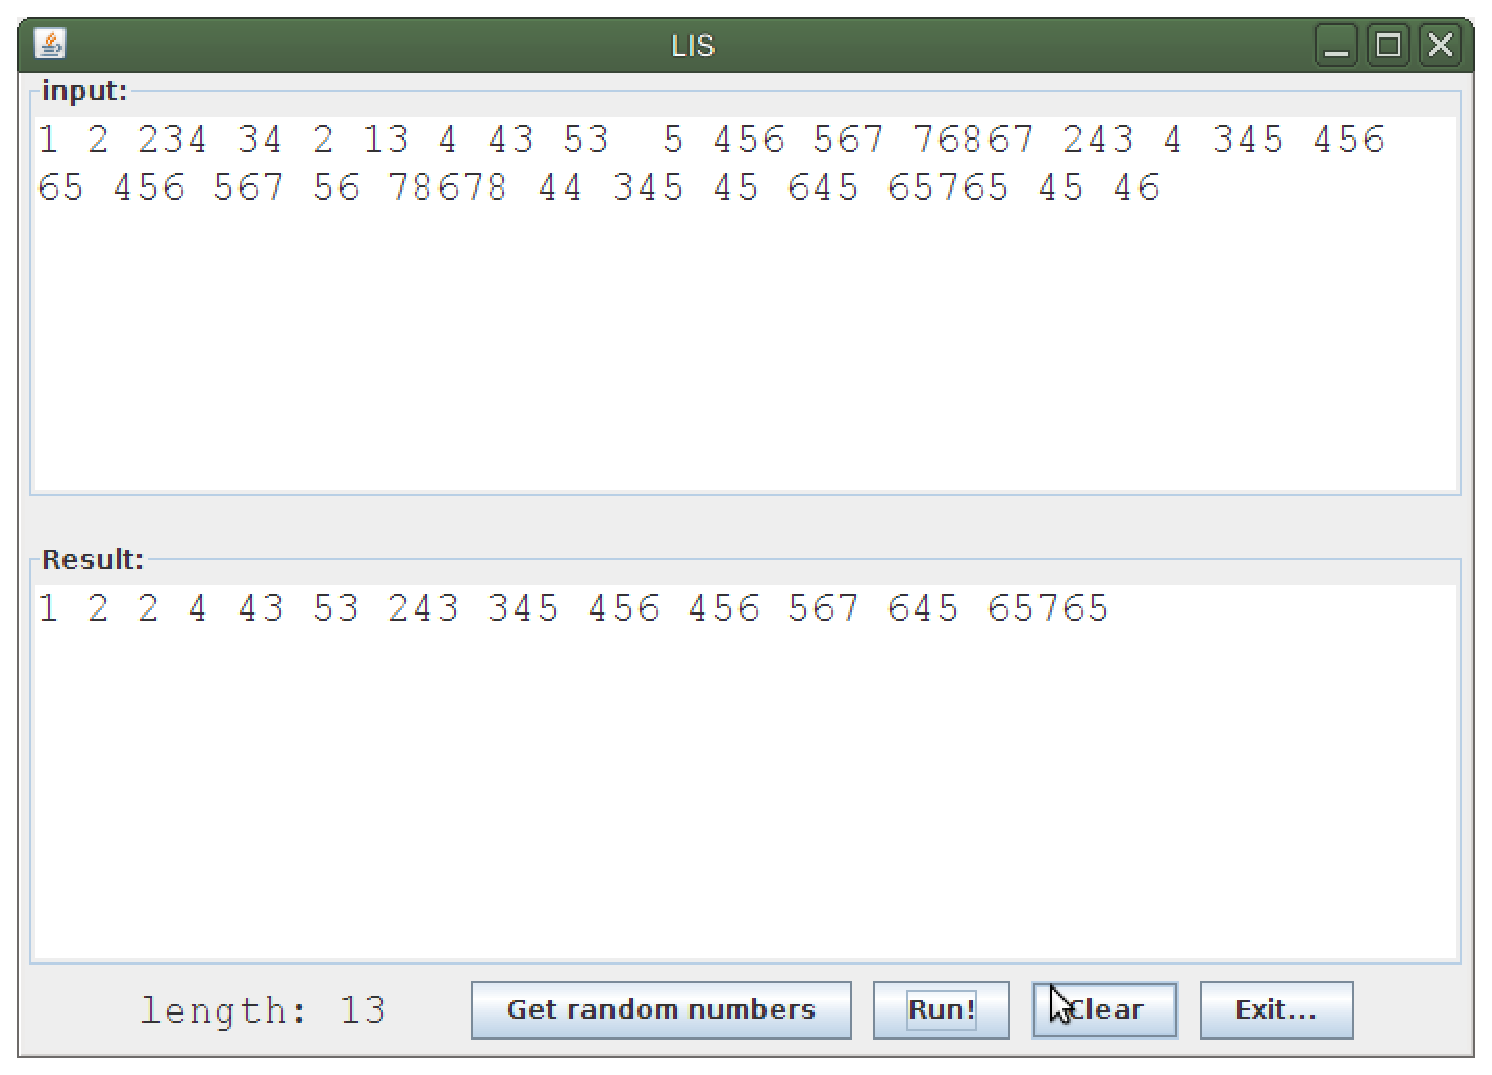
\includegraphics[height=8cm, width=11cm]{LIS.eps}
\end{figure}

\section{Problem 15-1 bitonic tours}

\begin{enumerate}
	\item 将所有的点按照x坐标从小到大排序。时间复杂度为$O(nlgn)$。排许后用序列
		$p_1, P_2, p_3 ... p_n$表示。
	\item 定义从$p_i$到$p_j$之间的双调路径$d(i,j)$为:从$p_i$开始,严格的向左走,
		直到$p_1$,然后严格的向右走直到$p_j$。途中经过$p_1$到$p_{max(i,j)}$
		之间的所有点一次其只一次。由于对称性,只考虑$i \ge j$的情况。定义
		$\Delta(i,j)$表示$p_i$和$p_j$之间的距离。
	\item 计算$d(i,j), i \ge j$,最基本的情况是$d(2,1)=\Delta(2,1)$。
		\begin{enumerate}
			\item 如果$j < i-1$,由于是严格的向左或向右走,从$p_j$出发向左走
				只能经过位置小于j的点。对于大于j小于i的点,由于要保持严格
				向右,因此只有一条路径。而$(p_i, p_{i-1})$一定在路径中。
				因此边$(p_i, p_{i-1})$一定在从$p_i$到$p_j$之间
				的双调路径上。那么$d(i,j)=d(i-1,j)+\Delta(i, i-1)$。
			\item 如果$j = i-1$,考虑在最短路径中最先连接的两个点,可以是$p_i$
				到$p_1$,$p_i$到$p_2$,...$p_i$到$p_{-2}$。所以
$d(i,j)=min(d(1,i-1)+\Delta(i,1),d(2,i-1)+\Delta(i,2),...,d(i-2,i-1)+\Delta(i,i-2))$
		\end{enumerate}
	\item 对于d[n][n],
$d(n,n)=min(d(1,n)+\Delta(n,1),d(2,n)+\Delta(n,2),...,d(n-1,n)+\Delta(n,n-1))$
		对于$i < n$的d[i][i],由于在整个计算中没有使用,因此不予计算。当然,如果计算
		d[i][i],那么程序将更简单。
\end{enumerate}
	
	算法如下:
\begin{verbatim}
    d[n][n]
    p[n] //存储所有的点。
    pre[n][n] = {-1}//保存计算信息,用于构造路径。
    按x坐标对p中的点进行排序。
    d[2][1] = distance(p[2], p[1])
    for(i从1到n)
        //j < i-1
        for(j从1到i-2)
            d[i][j]=d[i-1][j]+distance(p[i], p[i-1])
            pre[i][j]=i-1
        //j = i-1
        d[i][i-1] = d[1][i-1] + distance(p[1], p[i])
        pre[i][i-1]=1
        for(k从2到i-2)
            tmp = d[k][i-1] + distance(p[k], p[i])
            if(tmp > d[i][i-1])
                d[i][i-1] = tmp
                pre[i][i-1]=k
    d[n][n] = d[1][n] + distance(p[1], p[n])
    for(k从2到i-2)
        tmp = d[k][n] + distance(p[k], p[n])
        if(tmp > d[n][n])
            d[n][n] = tmp
            pre[n][n]=k
    d[n][n]中存储最终结果。
    
    path //存储最短路径的一半
    i = n, pre_i = n
    j = n, pre_j = n
    while(pre[i][j] != -1)
        if(j == i - 1)
            i = pre_i - 1
        将边(p[pre[i][j]], p[j])加入path中
        pre_i = i, pre_j =j
        i=pre[i][j]
    
\end{verbatim}
	外循环要n次,两个内循环都是i-2次,因此上面的算法的时间复杂度是$O(n^2)$。通过一个pre
数组记录每次构造d[i][j]的值所使用的d[k][j]的k。通过这个数组可以构造出整个路径的一半,也就是
从n到1的路径,另一半可以根据双调性很容易的构造出来。构造路径的时间复杂度是$O(n)$。
	
	参考原文如图\ref{btsp}
\begin{figure}[htbp]
\centering
\caption{双调旅行商问题}
\label{btsp}
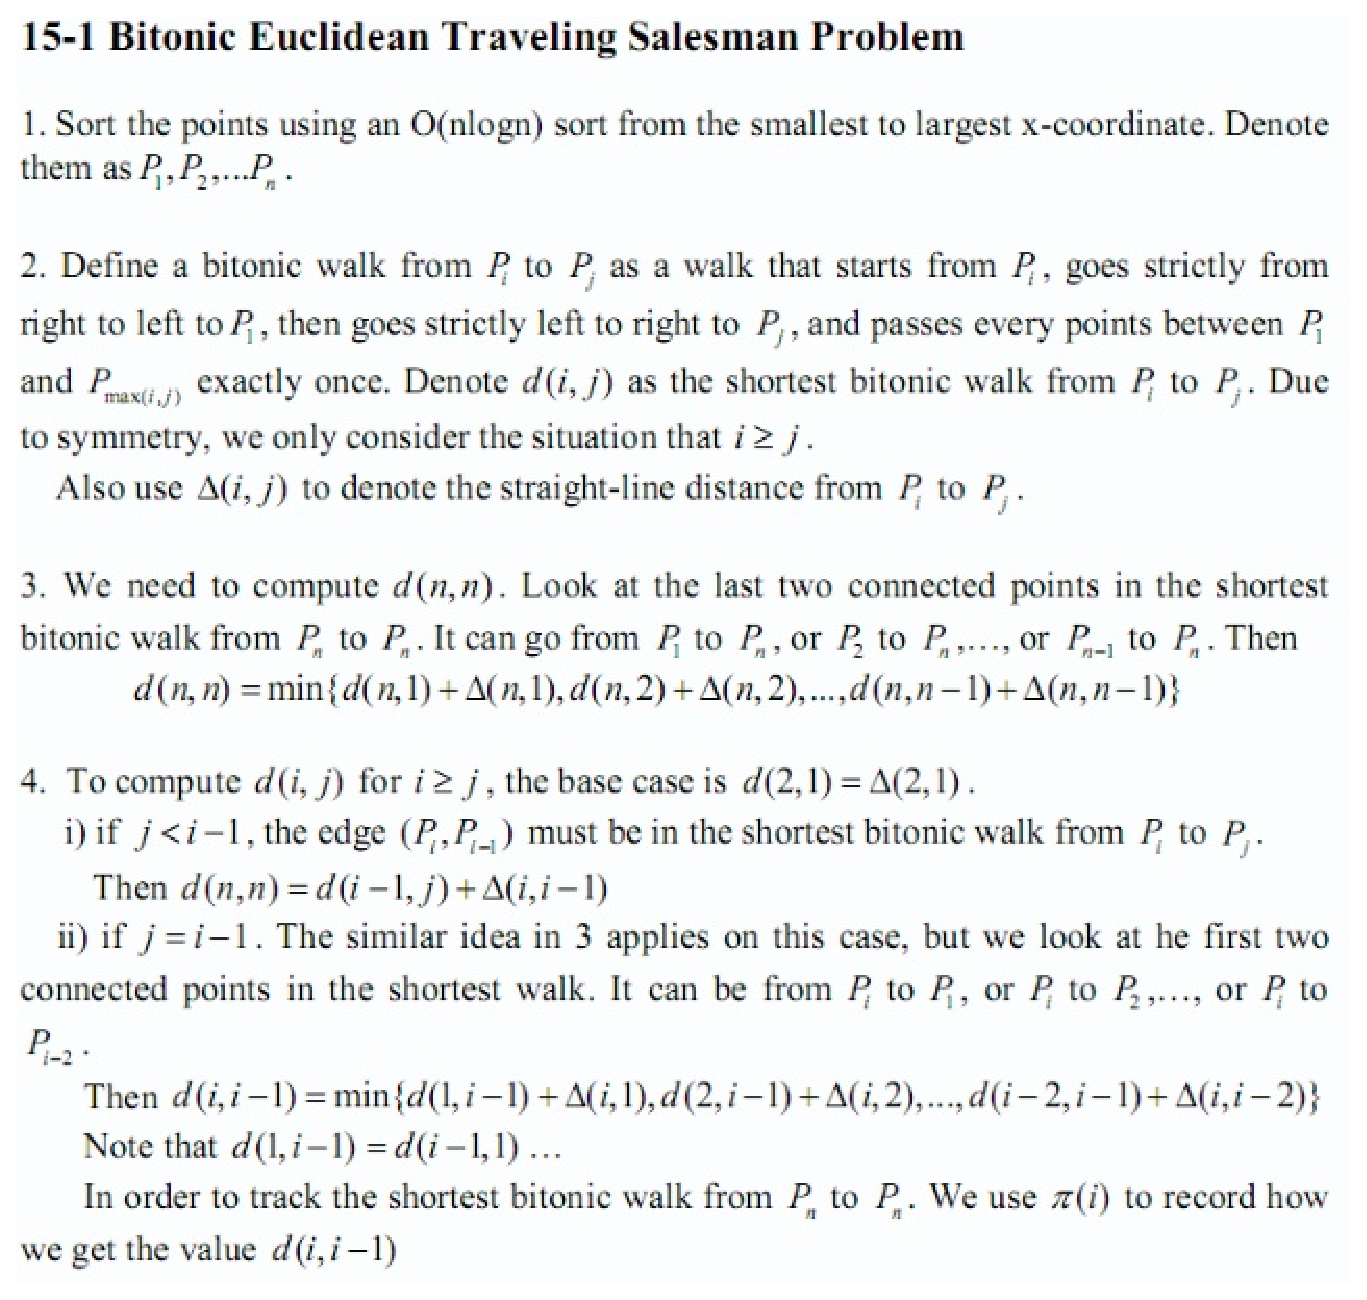
\includegraphics[height=9cm, width=10cm]{btsp.eps}
\end{figure}

\section{Problem 15-6 checker}

用一个n×n的二维数组c表示checkerboader。那么,对于格子c[i][j],checker只可能从c[i][j-1],
c[i-1][j-1]和c[i+1][j-1]三个格子移动过来。用一个二维数组b表示到达每个格子所能获得的最大钱数。
b[i][j]表示checker到达c[i][j]时所能获得的最大钱数。对每一个格子进行编号,用i*n+j表示,编号
之后便于查找p(x,y)的值。递推方程如下:
\begin{align*}
                     b[i][j]=max(b[i-1][j]+p((i-1)*n+j, i*n+j)\\
                     		,b[i-1][j-1]+p((i-1)*n+j-1, i*n+j)\\
                     		,b[i-1][j+1]+p((i+1)*n+j+1, i*n+j))
\end{align*}

算法如下:
\begin{verbatim}
    maxValue = -1
    b存储checker到达每个格子所得到的最大值。
    for(i=1; i < n; ++i)
        for(j=0; j < n; ++j)
            //对于超出边界的点,不与考虑。
            //但是,也可以在checkerboader的周围设置一个“围墙”。
            //对与围墙上的点,p(x,y)总是负无穷大,这样在下面的代码
            //中就不需要判断格子是否超出边界。
            b[i][j] = max(b[i-1][j]+p((i-1)*n+j, i*n+j)
                        ,b[i-1][j-1]+p((i-1)*n+j-1, i*n+j)
                        ,b[i-1][j+1]+p((i+1)*n+j+1, i*n+j));

    for(i=0; i < n; ++i)
        if(maxValue < b[n-1][i])
        maxValue = b[n-1][i]
\end{verbatim}
	
外层循环和内层循环分别是n-1次和n次,因此算法的复杂度是$O(n^2)$。
\end{document}
